% ==========================================================
% PneumoFusionNet — Term Project Report (Trimester 8)
% IIT Guwahati | B.Sc. Data Science & AI
% Ashutosh Yadav (Roll: 23035010693)
% ==========================================================

\documentclass{article}
\usepackage{spconf,amsmath,amssymb,graphicx,hyperref}
\usepackage{booktabs,enumitem,needspace,tikz,xcolor,tcolorbox}
\usetikzlibrary{arrows.meta,positioning}

\hypersetup{colorlinks=true,linkcolor=blue!70!black,
            citecolor=blue!70!black,urlcolor=teal}
\tcbuselibrary{skins}
\definecolor{successgrn}{RGB}{39,174,96}
\definecolor{alertred}{RGB}{192,57,43}

% Tighten vertical spacing globally
\setlength{\parskip}{1pt}
\setlength{\topsep}{2pt}
\setlength{\partopsep}{0pt}

\def\x{{\mathbf x}}
\def\L{{\cal L}}

% ------------------------------------------------------------------
\title{PneumoFusionNet: A Multimodal Deep Learning Framework\\
for Pneumonia Detection Using Chest X-Rays and Clinical Reports}

\name{Ashutosh Yadav (Roll Number: 23035010693)}

\address{
  Term Project Report (Trimester 8)\\[0.2em]
  B.Sc.\ (Honours) Data Science and Artificial Intelligence\\
  Indian Institute of Technology Guwahati, India \quad
  \texttt{ashutosh@op.iitg.ac.in}
}

% ==========================================================
\begin{document}
\ninept
\maketitle

% ==========================================================
\begin{abstract}
This report presents \textbf{PneumoFusionNet}, a multimodal deep learning framework
for pneumonia diagnosis, inspired by Yu et al.~\cite{frontiers2025pneumofusion} and
built on the restricted \textbf{MIMIC-CXR} hospital dataset.
\textbf{Stage~0:} Architecture validated on public datasets (Kaggle: 92\% accuracy;
IU dataset: multimodal pipeline prototype).
\textbf{Stage~1:} MIMIC-CXR selected after comprehensive dataset search; access
required CITI training and a PhysioNet Data Use Agreement (DUA). A 139-sample
pilot (ResNet50\,+\,DSC\,+\,GCSA) showed leakage-free text fusion yielding
\textbf{+3.7\% AUC} over the image-only model.
\textbf{Stage~2:} Scaling to 1,989 PA-only images, the identical architecture
\textbf{failed} (AUC\,=\,0.713, Accuracy\,=\,66.2\%), proving ImageNet-pretrained
ResNet50 is insufficient at clinical scale.
\textbf{Conclusion:} The project pivots to DenseNet-121 with domain-specific
CXR pretraining for the final stage.

\textbf{Index Terms---} Multimodal Deep Learning, MIMIC-CXR, Bio\_ClinicalBERT,
ResNet50, Label Leakage, Pneumonia Detection.
\end{abstract}

\begin{keywords}
Pneumonia Detection, Multimodal Learning, MIMIC-CXR, ResNet50, DSC, GCSA
\end{keywords}

% ==========================================================
\section{Introduction}
% ==========================================================

Pneumonia causes $\sim$2.5 million deaths annually~\cite{who2023}. Chest
radiography (CXR) is the primary diagnostic tool, yet visual ambiguity
makes interpretation challenging even for experienced radiologists.
Image-only AI models~\cite{rajpurkar2017chexnet} ignore clinical context;
adding radiology report text could help, but introduces a critical trap.

\begin{tcolorbox}[colback=red!4!white,colframe=red!55!black,
  title=Label Leakage,fonttitle=\small\bfseries,
  top=3pt,bottom=3pt,left=4pt,right=4pt]
\small
Every report ends with an \textbf{IMPRESSION} section stating the final diagnosis.
If seen during training, the model memorises the answer.
\textcolor{successgrn}{\checkmark}~\textbf{INDICATION / FINDINGS} --- retained.\quad
\textcolor{alertred}{\textbf{$\times$}~\textbf{IMPRESSION}} --- stripped completely.
\end{tcolorbox}

This project builds PneumoFusionNet on restricted MIMIC-CXR~\cite{johnson2019mimic}.
Sections 2--6 cover the full pipeline; Section~7 concludes.

% ==========================================================
\section{Stage 0: Architecture Validation on Public Datasets}
% ==========================================================

\subsection{Pilot Architecture: ResNet50 + DSC + GCSA}

\textbf{ResNet50}~\cite{he2016resnet} (ImageNet pretrained) extracts features;
its first convolutional layer is averaged for grayscale; first seven children frozen.
\textbf{DSC} compresses 2048$\to$1024 channels with $\sim$50\% fewer parameters:
\vspace{-2pt}
\begin{equation}
  \text{DSC}(\mathbf{X})=\text{BN}\!\left(\text{ReLU}\!\left(
    \mathbf{W}_{1\times1}\ast(\mathbf{W}_{dw}\circledast\mathbf{X})
  \right)\right) \label{eq:dsc}
\end{equation}
\vspace{-6pt}

\textbf{GCSA} combines channel and spatial attention:
\vspace{-4pt}
\begin{align}
  \mathbf{A}_{ch}&=\sigma\!\bigl(\text{MLP}(\text{AvgPool})+\text{MLP}(\text{MaxPool})\bigr)\label{eq:ach}\\
  \mathbf{A}_{sp}&=\sigma\!\bigl(\text{Conv}_{7\times7}([\text{AvgCh};\text{MaxCh}])\bigr)\label{eq:asp}\\
  \hat{\mathbf{X}}&=\mathbf{X}\cdot\mathbf{A}_{ch}\cdot\mathbf{A}_{sp}\label{eq:gcsa}
\end{align}
\vspace{-4pt}

\subsection{Public Dataset Results}

\begin{table}[h]
\centering
\caption{Stage 0: Results on public datasets.}
\label{tab:stage0}
\resizebox{\columnwidth}{!}{%
\begin{tabular}{llll}
\toprule
\textbf{Notebook} & \textbf{Dataset} & \textbf{Purpose} & \textbf{Result}\\
\midrule
\texttt{v1\_Basic\_Image\_Model}  & Kaggle CXR & Sanity check    & $\sim$92\% Acc.\\
\texttt{v2\_Enhanced\_GCSA\_DSC}  & Kaggle CXR & DSC+GCSA valid. & 92\% Acc., F1\,=\,0.91\\
\texttt{v3-1-iu-multimodal-image} & IU X-Ray   & Image baseline  & Pipeline $\checkmark$\\
\texttt{v3-2-iu-multimodal-text}  & IU X-Ray   & Image+text e2e  & Pipeline $\checkmark$\\
\bottomrule
\end{tabular}%
}
\end{table}

\noindent\textit{Caveat:} 92\% on Kaggle confirms the code is correct---not
clinical readiness. Kaggle data is pre-cleaned, balanced, and far easier than
real hospital data.

% ==========================================================
\section{Dataset Search and MIMIC-CXR Access}
% ==========================================================

No public dataset simultaneously provides CXR images, clinical history, and
full radiology reports (FINDINGS + IMPRESSION). After evaluating Kaggle, IU,
NIH ChestX-ray14, CheXpert, and PadChest, we selected
\textbf{MIMIC-CXR-JPG v2.0.0}~\cite{johnson2019mimic}---377,110 radiographs
from 65,379 patients, each paired with structured reports. Key differences
from public datasets: restricted access (CITI + DUA required),
real 5.6:1 class imbalance, mixed PA/AP/Lateral views, and CheXpert NLP
auto-labels. MIMIC-CXR is \textbf{not publicly downloadable}; access required
completing the CITI Program ethics training and signing a PhysioNet
Data Use Agreement (DUA). All data was handled strictly per the DUA terms.

% ==========================================================
\section{Methodology: Anti-Leakage Pipeline}
% ==========================================================

\subsection{Data Preparation}

We built \texttt{rebuild\_dataset\_findings.py} to process each radiology report:
(1) parse into named sections; (2) \textbf{retain} INDICATION and FINDINGS;
(3) \textbf{strip} IMPRESSION and CONCLUSION; (4) export filtered text to CSV.
Three versioned CSVs manage the pipeline:
\texttt{mimic\_dataset.csv} (image-only, 139 rows),
\texttt{mimic\_multimodal\_dataset.csv} (image + raw text), and
\texttt{mimic\_multimodal\_dataset\_v3.csv} (image + leakage-free text).

\subsection{System Architecture}

\begin{figure}[h]
\centering
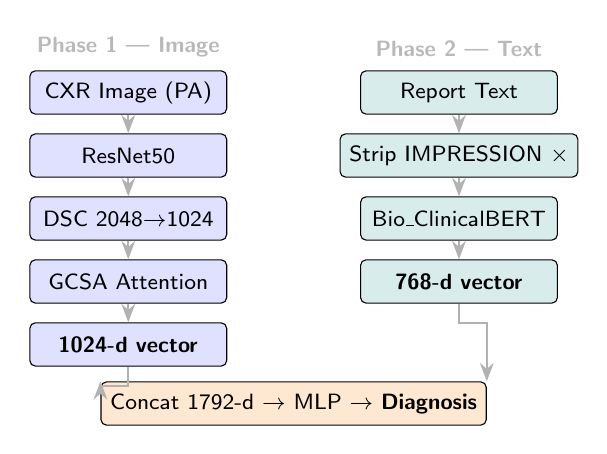
\begin{tikzpicture}[
  imgbox/.style={draw,rounded corners=2pt,fill=blue!12,align=center,
                 minimum height=0.55cm,minimum width=2.5cm,font=\footnotesize\sffamily},
  txtbox/.style={draw,rounded corners=2pt,fill=teal!15,align=center,
                 minimum height=0.55cm,minimum width=2.5cm,font=\footnotesize\sffamily},
  fusbox/.style={draw,rounded corners=2pt,fill=orange!18,align=center,
                 minimum height=0.55cm,minimum width=2.5cm,font=\footnotesize\sffamily},
  arr/.style={-Stealth,thick,gray!60},
  lbl/.style={font=\footnotesize\bfseries\sffamily,text=gray!55}
]
\node[imgbox](img) at (0,4.2){CXR Image (PA)};
\node[imgbox](res) at (0,3.4){ResNet50};
\node[imgbox](dsc) at (0,2.6){DSC 2048$\to$1024};
\node[imgbox](gcsa)at (0,1.8){GCSA Attention};
\node[imgbox](iemb)at (0,1.0){\textbf{1024-d vector}};

\node[txtbox](rep)  at (4.2,4.2){Report Text};
\node[txtbox](strip)at (4.2,3.4){Strip IMPRESSION $\times$};
\node[txtbox](bert) at (4.2,2.6){Bio\_ClinicalBERT};
\node[txtbox](temb) at (4.2,1.8){\textbf{768-d vector}};

\node[fusbox](cat) at (2.1,0.25){Concat 1792-d $\to$ MLP $\to$ \textbf{Diagnosis}};

\node[lbl,above=0.05cm of img]{Phase 1 --- Image};
\node[lbl,above=0.05cm of rep]{Phase 2 --- Text};

\draw[arr](img)--(res);\draw[arr](res)--(dsc);
\draw[arr](dsc)--(gcsa);\draw[arr](gcsa)--(iemb);
\draw[arr](rep)--(strip);\draw[arr](strip)--(bert);
\draw[arr](bert)--(temb);
\draw[arr](iemb.south)--++(0,-0.25)-|(cat.north west);
\draw[arr](temb.south)--++(0,-0.25)-|(cat.north east);
\end{tikzpicture}
\vspace{-4pt}
\caption{PneumoFusionNet: image branch (1024-d) + leakage-free text branch
(768-d) concatenated and classified by an MLP.}
\label{fig:pipeline}
\end{figure}

\vspace{-2pt}
Bio\_ClinicalBERT~\cite{alsentzer2019bert} (pretrained on MIMIC-III clinical
notes) encodes FINDINGS + INDICATION into a 768-d \texttt{[CLS]} vector;
last two layers fine-tuned. The fusion MLP predicts:
\vspace{-3pt}
\begin{equation}
  \hat{y}=W_2\cdot\text{ReLU}(W_1\cdot[\mathbf{v}_{img}\|\mathbf{t}_{text}]+b_1)+b_2
  \label{eq:fusion}
\end{equation}

% ==========================================================
\section{Stage 1: MIMIC-CXR Pilot Study (139 Samples)}
% ==========================================================

\textbf{Dataset:} 139 samples (118 Normal, 21 Pneumonia; 5.6:1 imbalance) from
MIMIC-CXR P10; all view types (PA, AP, Lateral); row-level 70/15/15 split
(97 train / 21 val / 21 test).

\begin{table}[h]
\centering
\caption{Pilot results (139 samples, ResNet50+DSC+GCSA).}
\label{tab:pilot}
\resizebox{\columnwidth}{!}{%
\begin{tabular}{clccc}
\toprule
\textbf{Ph.} & \textbf{Configuration} & \textbf{AUC} & \textbf{Acc.} & \textbf{F1}\\
\midrule
1   & Image only, imbalanced (118:21)   & 0.667          & 76.2\%          & 0.430\\
1.1 & Image only, balanced (21:21)      & 0.917          & 85.7\%          & 0.857\\
2   & Image+Text, imbalanced (118:21)   & \textbf{0.704} & \textbf{81.0\%} & 0.447\\
2.1 & Image+Text, balanced (21:21)      & 0.917          & 71.4\%          & 0.708\\
\midrule
\multicolumn{2}{l}{\textit{Gain (Ph.2 vs.~Ph.1, imbalanced)}}
  & $+0.037$ & $+4.8\%$ & $+0.017$\\
\bottomrule
\end{tabular}%
}
\end{table}

On the realistic imbalanced split, leakage-free text fusion improved AUC
by \textbf{+3.7\%} and accuracy by +4.8\%. This is genuine signal from
FINDINGS/INDICATION --- IMPRESSION was never seen by the model.

\textbf{Statistical Honesty (N=7 problem).} Balanced test set had 7 samples;
one error $\equiv$ 14.28\% swing. Using $CI_{95\%}=p\pm 1.96\sqrt{p(1-p)/N}$:
Phase~1.1: $85.7\%\pm 25.9\% \to [59.8\%,100\%]$;
Phase~2.1: $71.4\%\pm 33.5\% \to [38.0\%,100\%]$.
Fisher's Exact Test yields $p\approx 1.000$ --- the difference is
\textbf{statistically insignificant}. AUC\,=\,0.917 on 7 samples is meaningless.

\textbf{Pilot limitations:} (1)~View-type confound (PA/AP/Lateral mixed);
(2)~row-level split risks patient identity leakage;
(3)~N=7 test set is statistically meaningless.

% ==========================================================
\section{Stage 2: Scale-Up and Architecture Failure}
% ==========================================================

\textbf{Dataset:} 1,989 PA-only images (1,062 Normal + 927 Pneumonia).
Two fixes from pilot: \textbf{PA-only filtering} (eliminates view-type confound)
and \textbf{patient-level} \texttt{GroupShuffleSplit} by \texttt{subject\_id}
(zero patient overlap): 1,401 train / 295 val / 293 test.

We ran the \emph{identical} ResNet50\,+\,DSC\,+\,GCSA on the scale-up dataset
(Notebook: \texttt{Phase-1.1-pilot\_arch\_scaleUp\_ResNet\_DSC\_GCSA.ipynb}):

\begin{table}[h]
\centering\small
\setlength{\tabcolsep}{6pt}
\caption{Pilot architecture at two scales (pilot $N{=}7$ vs.\ scale-up $N{=}293$).}
\label{tab:failure}
\begin{tabular}{lcc}
\toprule
\textbf{Metric} & \textbf{Pilot (N=7)} & \textbf{Scale-Up (N=293)}\\
\midrule
AUC-ROC   & 0.917 {\small(unreliable)} & \textbf{0.713}\;$\downarrow$\\
Accuracy  & 85.7\%                     & \textbf{66.2\%}\;$\downarrow$\\
Sensitivity & ---                      & 69.9\%\\
Specificity & ---                      & 63.5\%\\
F1 (macro)& 0.857                      & \textbf{0.660}\\
\midrule
\multicolumn{3}{l}{\small CM (N=293): TN=108, FP=62, FN=37, TP=86}\\
\bottomrule
\end{tabular}
\end{table}

\textbf{Root Cause:}
(1)~\textit{ImageNet domain mismatch} --- ResNet50 pretrained on 1.2M natural
images cannot detect subtle CXR opacities and air bronchograms;
(2)~\textit{Insufficient training data} --- 1,401 images cannot override
ImageNet-biased representations;
(3)~\textit{Clinical complexity} --- real MIMIC-CXR contains medical devices,
overlapping anatomy, and variable scanner exposures absent from Kaggle.

% ==========================================================
\section{Discussion and Conclusion}
% ==========================================================

\textbf{Key findings:}
\begin{enumerate}[noitemsep,leftmargin=*,topsep=2pt]
  \item \textbf{Public $\neq$ clinical.} 92\% on Kaggle collapsed to 66.2\% on
        MIMIC-CXR. Public-dataset accuracy gives false confidence.
  \item \textbf{Leakage-free text works.} +3.7\% AUC from FINDINGS/INDICATION
        (IMPRESSION never seen) is genuine diagnostic signal.
  \item \textbf{Small test sets are meaningless.} AUC\,=\,0.917 on N=7 has
        CI\,=\,[59.8\%,100\%]; the honest N=293 answer is AUC\,=\,0.713.
  \item \textbf{Architecture must be replaced.} ResNet50\,+\,DSC\,+\,GCSA fails
        at clinical scale due to ImageNet domain mismatch.
\end{enumerate}

\textbf{Limitations:} Single institution; binary classification (14+ real findings);
no external validation; text fusion not evaluated at scale.

\textbf{Part 2 Roadmap:}
\begin{enumerate}[noitemsep,leftmargin=*,topsep=2pt]
  \item \textbf{DenseNet-121}~\cite{huang2017densenet} (\texttt{torchxrayvision},
        pretrained on $>$500K real CXRs) --- directly fixes the domain-mismatch.
  \item Multimodal fusion at scale: Bio\_ClinicalBERT + cross-attention.
  \item Phase~3: MIMIC-IV lab values (WBC, CRP, Procalcitonin).
  \item 5-fold GroupKFold cross-validation for robust evaluation.
\end{enumerate}

\textbf{Artifacts:} Code at \href{https://github.com/Ashutosh-yadav0001/PneumoFusionNet}
{\texttt{github.com/Ashutosh-yadav0001/PneumoFusionNet}}; Stage~0 notebooks in
\texttt{model\_experiments/}; Stage~1 in \texttt{mimic/mimic\_pilot\_139/Notebooks/};
Stage~2 notebook \texttt{Phase-1.1-pilot\_arch\_scaleUp\_ResNet\_DSC\_GCSA.ipynb};
MIMIC-CXR data restricted (PhysioNet DUA + CITI required).


% ==========================================================
\clearpage
\small
\begin{thebibliography}{9}

\bibitem{frontiers2025pneumofusion}
S.~Yu et al., ``A multi-modal deep learning solution for precise pneumonia
diagnosis: the PneumoFusion-Net model,'' \emph{Frontiers in Physiology},
vol.~16, Art.~1512835, Mar.\ 2025.
DOI: \href{https://doi.org/10.3389/fphys.2025.1512835}{10.3389/fphys.2025.1512835}

\bibitem{rajpurkar2017chexnet}
P.~Rajpurkar et al., ``CheXNet: Radiologist-Level Pneumonia Detection on Chest
X-Rays with Deep Learning,'' \emph{arXiv:1711.05225}, 2017.

\bibitem{johnson2019mimic}
A.~E.~W.~Johnson et al., ``MIMIC-CXR, a de-identified publicly available
database of chest radiographs with free-text reports,''
\emph{Scientific Data}, vol.~6, no.~317, 2019.

\bibitem{alsentzer2019bert}
E.~Alsentzer et al., ``Publicly Available Clinical BERT Embeddings,''
\emph{arXiv:1904.03323}, 2019.

\bibitem{he2016resnet}
K.~He, X.~Zhang, S.~Ren, and J.~Sun, ``Deep Residual Learning for Image
Recognition,'' \emph{Proc.\ IEEE CVPR}, 2016, pp.~770--778.

\bibitem{huang2017densenet}
G.~Huang, Z.~Liu, L.~van~der~Maaten, and K.~Q.~Weinberger,
``Densely Connected Convolutional Networks,''
\emph{Proc.\ IEEE CVPR}, 2017, pp.~4700--4708.

\bibitem{who2023}
World Health Organization, ``Pneumonia,'' \emph{WHO Fact Sheet}, 2023.
\url{https://www.who.int/news-room/fact-sheets/detail/pneumonia}

\end{thebibliography}

\end{document}
